\section{Preisstabilität}
\begin{multicols}{2}
   \subsection{Inflation}
Eine Inflation bedeutet eine permanente Steigerung des Preisniveaus.\\
Auslöser ist eine einmalige Steigerung des Preisniveaus durch
\begin{itemize}
	\item einen expansiven Nachfrageschock
	\item oder einen negativen Angebotsschock.
\end{itemize}
Ob dies zu einer Inflation führt, hängt von den Inflationserwartungen der Haushalte und Unternehmen sowie von der Reaktion der Geldpolitik der Zentralbank ab.\\
Bei einer Erhöhung der Geldmenge sinkt der Zinssatz und gleichzeitig steigt die Nachfrage nach Geld.
\vfill\null 
\columnbreak
\includegraphics[width=\linewidth]{images/Inflationswirkung}
Bei einer Inflation profitieren alle Schuldner wie z.B. Staaten, da die Realschuld mit der Inflationsrate abnimmt.
\end{multicols}

\begin{multicols}{2}
\subsubsection{Expansiver Nachfrageschock als Inflationsauslöser}
Geringe Ausweitung des realen BIP, aber deutliche Erhöhung des Preisniveaus (vorerst einmalige Preissteigerung). Ursache dafür einer der vier Faktoren: Staat, Haushalte, Firmen oder Exporte sein.
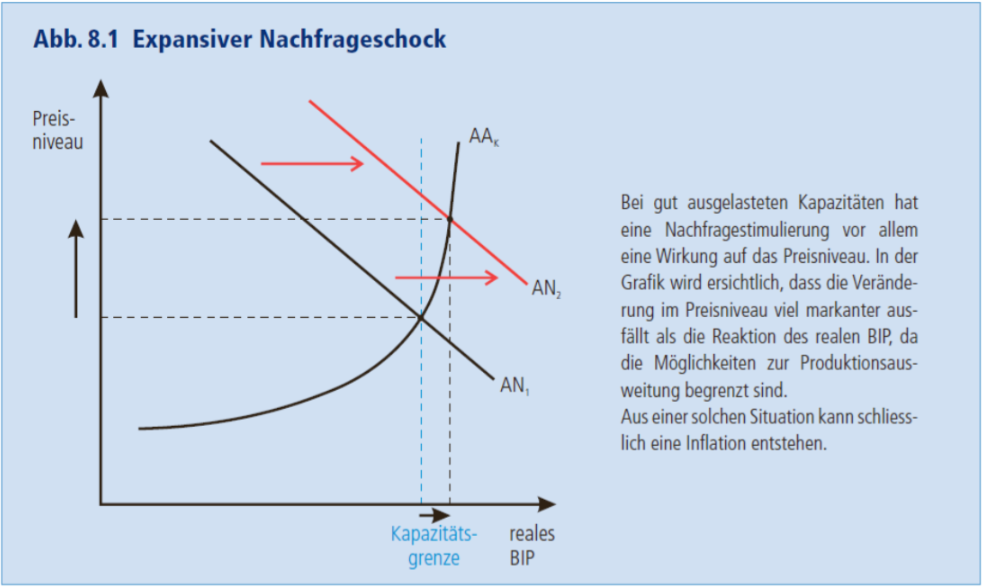
\includegraphics[width=\linewidth]{images/nachfrageschock.png}
\columnbreak
\subsubsection{Negativer Angebotsschock als Inflationsauslöser}
Gleichzeitiger Rückgang des realen BIP und Erhöhung des Preisniveaus (Stagflation) (vorerst einmalige Preissteigerung). Ursache dafür können z.B. höhere Löhne oder Unternehmenssteuern sein.
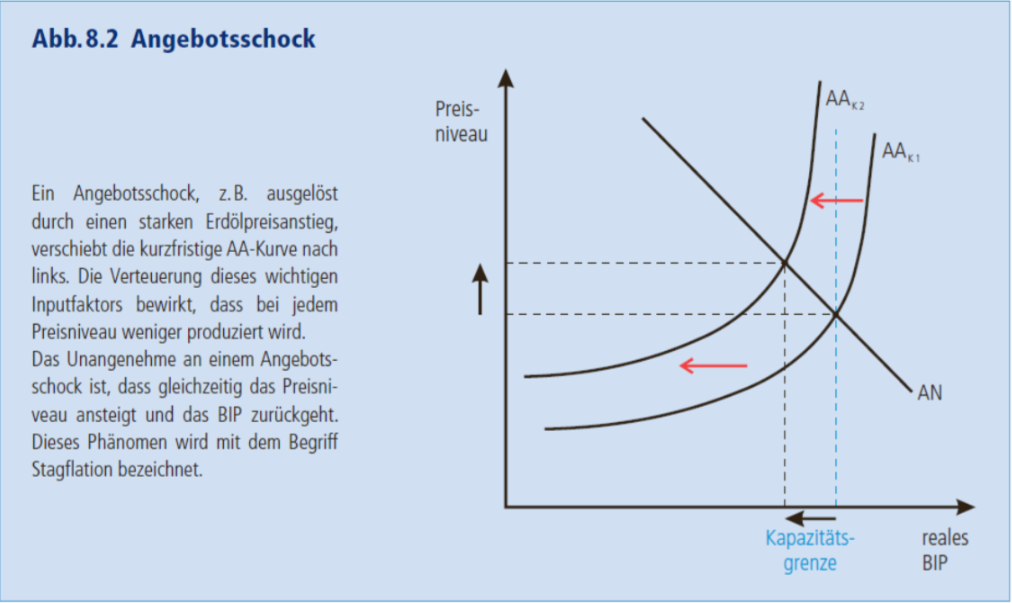
\includegraphics[width=\linewidth]{images/angebotsschock.png}
\end{multicols}

\vspace{-\baselineskip}
\subsubsection{Lohn-Preis-Spirale}
Erhöhtes Preisniveau durch einmaligen Schock.
\begin{itemize}
	\item[\-] 1. Sinkende Reallöhne der Haushalte
	\item[\-] 2. Diese fordern (Inflationserwartung) Steigerung der Nominallöhne, welche Erhöhung des Preisniveaus überkompensieren
	\begin{itemize}
		\item[\-] (Falls die Haushalte keine Inflationserwartung haben, werden sie nur eine Steigerung der Nominallöhne auf das alte (Real-)Lohnniveau verlangen. Damit entsteht keine Inflation.)
	\end{itemize}
	\item[\-] 3. Damit ergibt sich eine Steigerung der Reallöhne
	\item[\-] 4. Dies bedeutet für die Unternehmen eine Kostensteigerung
	\item[\-] 5. Die Unternehmen werden deshalb höhere Güterpreise verlangen
	\item[\-] 6. Damit erhöht sich wieder das Preisniveau (Zweitrundeneffekt)
	\item[\-] 1. ...
\end{itemize}
Befriedigt die Geldpolitik die erhöhte Nachfrage nach Geld 
(ausgelöst durch Erhöhung des allgemeinen Preisniveaus) mit einem erhöhten Geldangebot, besteht die Gefahr, dass eine Lohn-Preis-Spirale in Gang gesetzt wird.

\subsubsection{Quantitätsgleichung}
\begin{align*} 
    P \cdot Q &= M \cdot V\\
	\underbrace{Preisniveau \cdot reales \; BIP}_{\text nominales \; BIP} &= Geldmenge \cdot Geldumlaufgeschwindigkeit
\end{align*}
Geldumlaufgeschwindigkeit = Anzahl der Verwendungen einer Geldeinheit pro Jahr (in den weiteren Analysen als konstante Grösse betrachtet)

\subsection{Erhöhung der Geldmenge}
\begin{multicols}{2}
\textbf{langfristige Betrachtung:}\\
Das makroökonomische Modell zeigt, dass langfristig die Erhöhung der Geldmenge keinen Einfluss auf das reale BIP hat. Gemäss der Quantitätsgleichung führt dies nur zu einer proportionalen Erhöhung des Preisniveaus.\\
$\uparrow P \cdot Q = \uparrow M \cdot V$
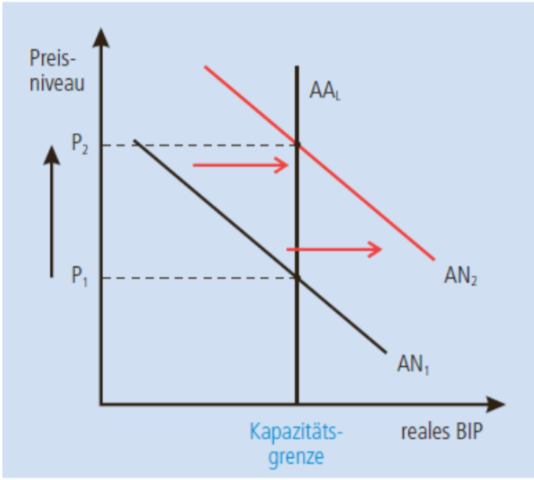
\includegraphics[width=\linewidth]{images/geldmengenerhoehung.png}
\vfill\null
\columnbreak
\textbf{kurzfristige Betrachtung:}\\
Fall 1:\\
Ausgangslage: Nicht ausgelastete volkswirtschaftliche Kapazität.\\
Input: Die Geldmenge wird erhöht.\\
Quantitätsgleichung: $\uparrow P \cdot \uparrow Q = \uparrow M \cdot V$\\
Also: $\Delta P < \Delta Q$\\
Fall 2:\\
Ausgangslage: Voll ausgelastete volkswirtschaftliche Kapazität.\\
Input: Die Geldmenge wird erhöht.\\
Quantitätsgleichung: $\uparrow P \cdot \uparrow Q = \uparrow M \cdot V$\\
Also: $\Delta P > \Delta Q$
\includegraphics[width=\linewidth]{images/Inflationswirkung}
\end{multicols}

\subsubsection{Die $"$Liquiditätsfalle$"$}
Folgender Sachverhalt liegt vor:\\
$P \cdot Q = \uparrow M \cdot \downarrow V$\\
Geld wird aus Gründen einer düsteren Zukunftseinschätzung gehortet statt ausgegeben (Liquiditätsfalle). Eine expansive Geldpolitik hat damit keine Auswirkung mehr auf das reale BIP (Weltwirtschaftskrise 1929). Keynes empfahl in dieser Situation den Einsatz der Fiskalpolitik durch den Staat.
\clearpage

\subsubsection{Geldmengenerhöhung: Fazit}
Hinter jeder Inflation steht letztlich eine Expansion der Geldmenge, welche grösser als die Zunahme des realen BIP ist.\\
Der Staat kann seine Ausgaben grundsätzlich auf drei Arten finanzieren:
\begin{itemize}
	\item Erhebung von Steuern
	\item Verschuldung
	\item "Drucken" von Geld
\end{itemize}
Während die ersten beiden Arten politisch nicht sehr attraktive Finanzierungsarten sind (Wählerverluste bzw. Fremdzinsen), ist die dritte Art letztlich nichts anderes als eine Form von $"$Steuer$"$ auf die Geldhaltung (Inflationssteuer). Dies setzt allerdings die Kooperation der Zentralbank voraus.

\subsubsection{Kosten einer moderaten Inflation}
\begin{multicols}{2}
\begin{itemize}
	\item Transaktionskosten (Viele kleine Bankabhebungen) 
	\item Kosten der Unsicherheit (Zinsen)
	\item Kosten aufgrund der Verzerrung der relativen Preise (Verwischung der Knappheitssignale, da sich Güterpreise unterschiedlich schnell anpassen)
	\item Kosten für Kreditgeber (Inflation frisst Realzinsen bzw. Kapital der Haushalte auf; Staat kann so seine Schulden abbauen)
	\item Kosten aufgrund der kalten Progression der Steuern (höheres Nominaleinkommen führt zur Einstufung in höhere Steuerklassen
	\item Inflation wird mit Verkleinerung der Geldmenge bekämpft, dadurch oftmals Rezession
\end{itemize}
\columnbreak
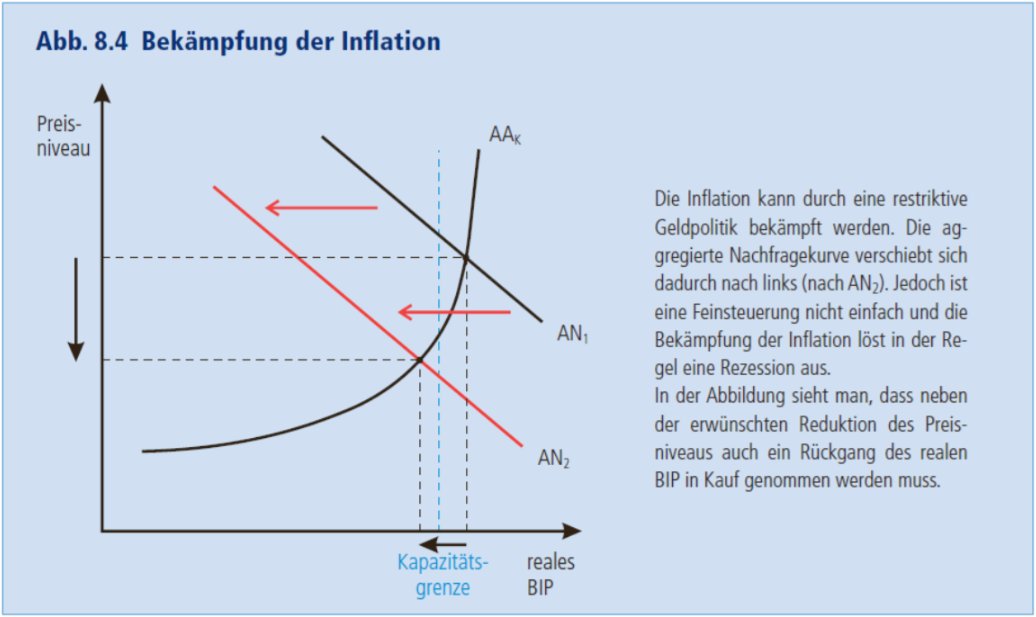
\includegraphics[width=\linewidth]{images/inflationsbekaempfung.png}
\end{multicols}

\subsubsection{Philips-Kurve}
\begin{multicols}{2}
\textbf{Kritik (Milton Friedman)}\\
Bei Vollbeschäftigung (ohne konjunkturelle Arbeitslosigkeit) gibt es langfristig keinen $"$trade off$"$ zwischen Inflation und Arbeitslosigkeit.
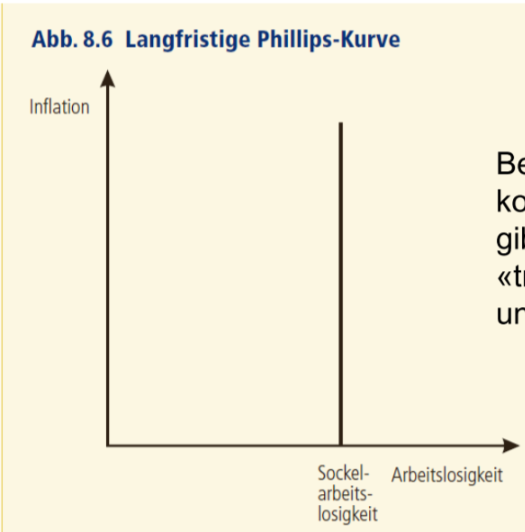
\includegraphics[width=0.5\linewidth]{images/philipskurve2.png}
\vfill\null
\columnbreak
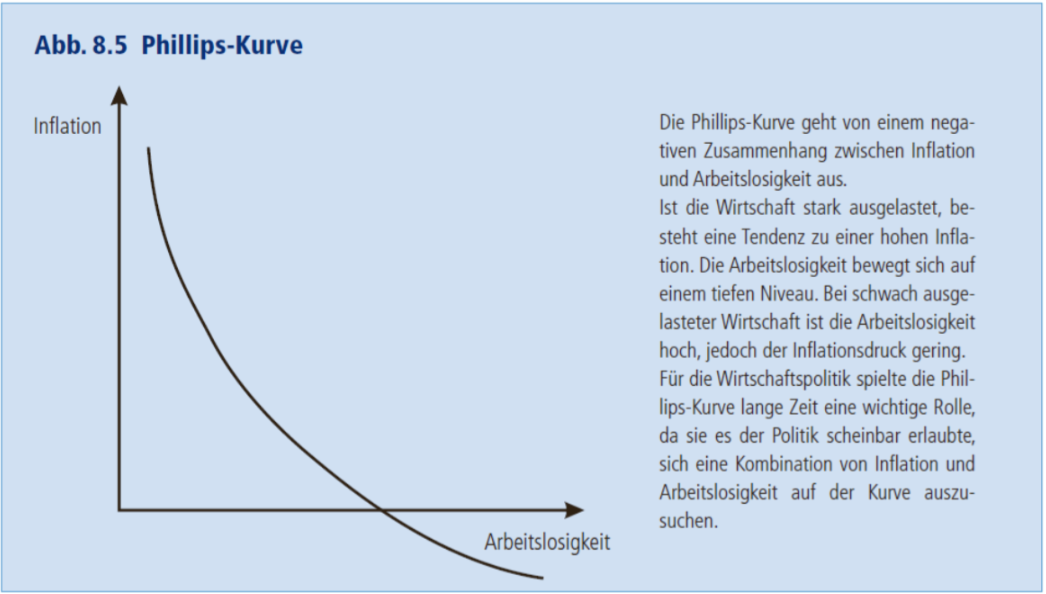
\includegraphics[width=\linewidth]{images/philipskurve.png}
\end{multicols}
\clearpage

\subsection{Deflation}
Eine Deflation bedeutet ein permanenter Rückgang des Preisniveaus.\\
Die Deflation ist dann schädlich, wenn diese auf einem Rückgang der aggregierten Nachfrage (AN) beruht. Ein Preisrückgang aufgrund einer Ausweitung des aggregierten Angebots (AA) führt zu keiner Deflation.\\
Eine einmal entstandenen Deflation ist ausgesprochen persistent und kann mithilfe der konventionellen Geldpolitik kaum mehr aus der Welt schaffen, weil alle erwarten, dass es günstiger wird und daher immer weiter zuwarten mit Konsum.

\begin{multicols}{2}
\subsubsection{Deflationärer Boom}
Ausgangslage: Voll ausgelastete volkswirtschaftliche Kapazität.\\
Input: Neue Technologien erlauben höhere Produktivität bei jedem Preisniveau.\\
Ergebnis: Senkung des Preisniveaus bei gleichzeitig höherem realen BIP $\rightarrow$ Deflationärer Boom!
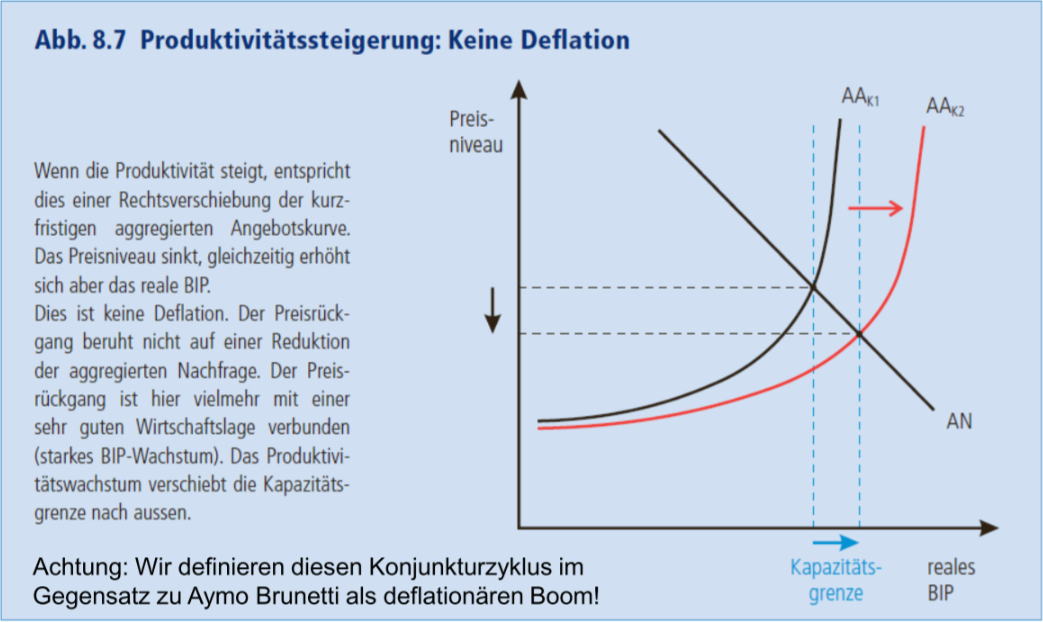
\includegraphics[width=\linewidth]{images/produktivitaetssteigerung.png}
\columnbreak
\subsubsection{Depression}
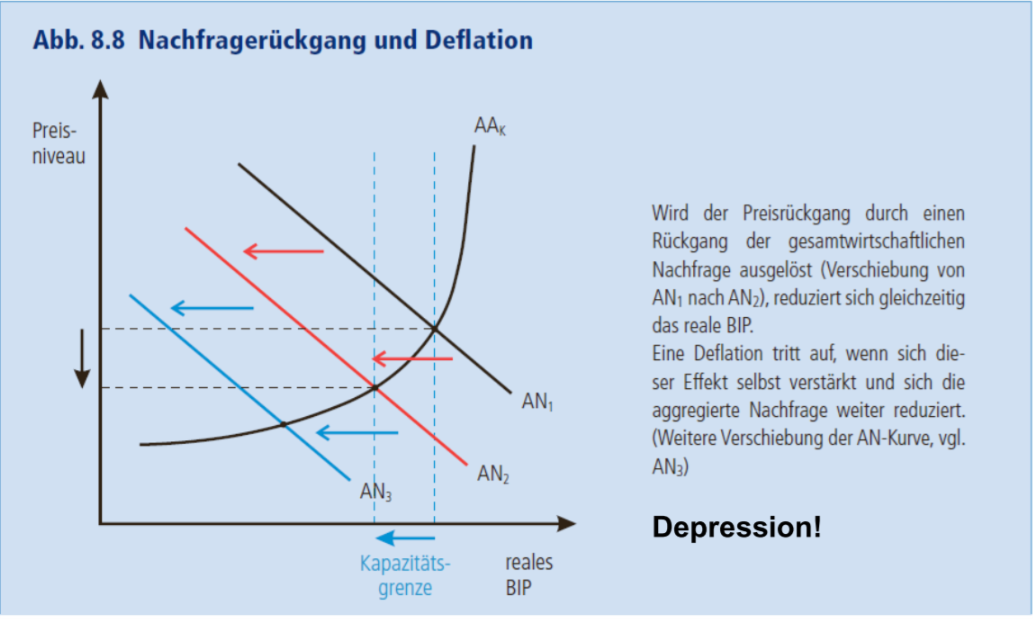
\includegraphics[width=\linewidth]{images/nachfragerueckgang.png}
\end{multicols}

\subsubsection{Folgen der Deflation}
\begin{itemize}
    \item Selbstverstärkende Wirkung
    \subitem Ausgelöst durch ausgeprägte Deflationserwartungen
    \item Hohe Realzinsen
    \subitem Realzins = Nominalzins (minimal 0\%) + erwartete Deflation
    \item Steigende Reallöhne
    \subitem Steigende Produktionskosten für Unternehmen
    \item Sinkende Bonität der Schuldner und Bankkrisen
    \subitem Kreditgeber gewinnen (Haushalte), Kreditnehmer verlieren (steigender Realwert der Schulden)
\end{itemize}

\subsubsection{Deflation: Fazit}
In der Regel wird Preisstabilität nicht als Wert zwischen -1\% und +1\% verstanden, sondern als Wert zwischen 0\% und 2\% (zur Verringerung der Gefahr einer Deflation).

\clearpage
\pagebreak